\documentclass[12pt,a4paper]{article}

% ---------------- Packages ----------------
\usepackage{amsmath, amssymb, amsfonts}
\usepackage{graphicx}
\usepackage{subcaption}
\usepackage{booktabs}
\usepackage{geometry}
\usepackage{hyperref}
\usepackage{xcolor}
\usepackage{siunitx}
\usepackage{tabularx}
\usepackage{makecell}
\usepackage{ragged2e}
\usepackage{placeins}

\geometry{margin=1in}
\graphicspath{{./}} % put your PNGs next to main.tex

\hypersetup{
  colorlinks=true,
  linkcolor=blue!60!black,
  citecolor=blue!60!black,
  urlcolor=blue!60!black
}

% ---------------- Title ----------------
\title{Non-Deterministic Unsupervised Neural Network Model:\\ HSEN vs VAE vs AE}
\author{Pranto Roy}
\date{September 2025}
\setlength{\parskip}{0.8em}
\setlength{\parindent}{0pt}
\begin{document}

\maketitle

% ---------------- Abstract ----------------
\begin{abstract}
\justifying
This study presents the \textit{Heteroscedastic Stochastic Embedding Network} (HSEN), a non-deterministic neural model for unsupervised dimensionality reduction and clustering on a kidney disease dataset. HSEN incorporates stochastic latent variables with a stability regularizer, balancing uncertainty and clusterability. We compare HSEN against a \textit{Variational Autoencoder} (VAE) baseline and a \textit{deterministic Autoencoder} (AE). Results show that HSEN achieves lower reconstruction error than VAE, higher trustworthiness (\num{0.997} vs. \num{0.687}), improved continuity (\num{0.866} vs. \num{0.143}), and stable clustering performance (stability NMI = \num{0.968}). While AE excels at raw reconstruction (MSE = \num{0.0055}), it lacks uncertainty estimation. Findings highlight the benefits of stochastic embeddings for robust unsupervised learning.
\end{abstract}

% ---------------- Introduction ----------------
\section{Introduction}
Unsupervised learning aims to extract patterns from unlabeled data, enabling discovery of hidden structure and representations without supervision. Non-deterministic neural models introduce stochasticity, which promotes manifold exploration and provides uncertainty estimates.

We investigate dimensionality reduction and clustering on a kidney disease dataset and propose \textbf{HSEN}, extending the VAE with a \emph{stability regularizer} that encourages multiple stochastic samples of the same input to be close in latent space. We compare HSEN with a VAE baseline and a deterministic AE. Our objectives are: (i) evaluate HSEN for dimensionality reduction and clustering, (ii) compare with AE and VAE, and (iii) quantify uncertainty and clustering stability.

% ---------------- Related Work ----------------
\section{Related Work}
Variational Autoencoders (VAE)~\cite{kingma2013auto} introduced stochastic latent embeddings via the reparameterization trick. On tabular datasets, VAEs may suffer from \emph{posterior collapse}, yielding weak latents. Deterministic autoencoders minimize reconstruction loss but cannot quantify uncertainty. Unsupervised deep embedding methods for clustering~\cite{xie2016unsupervised} and disentangling approaches such as $\beta$-VAE~\cite{higgins2016beta} inspired regularizers that improve geometry and interpretability. Our HSEN adds a simple stability term to the VAE objective, improving clusterability while retaining useful uncertainty.

% ---------------- Methodology ----------------
\section{Methodology}

\subsection{Dataset Analysis}
We use a kidney disease dataset with nine numeric features ($\sim$2300 samples). Preprocessing includes median imputation, standardization, and an 80/20 train--test split. No labels are used for training. Due to the lack of ground truth clusters, we report silhouette and \emph{stability} (NMI across $k$-means runs); ARI/NMI w.r.t.\ labels are omitted.

\subsection{Model Architectures}
\textbf{AE (deterministic baseline):} Encoder--decoder with deterministic latent $z$. Loss:
\[
\mathcal{L}_{AE} = \mathrm{MSE}(x,\hat{x}).
\]

\textbf{VAE (baseline):} Encoder outputs $(\mu,\log\sigma^2)$; reparameterization trick with KL regularization. Loss:
\[
\mathcal{L}_{VAE} = \mathrm{MSE}(x,\hat{x}) + \beta \cdot KL\!\left(q(z\mid x)\,\|\,p(z)\right).
\]

\textbf{HSEN (proposed):} As VAE, but sample $z_1,z_2$ per input and penalize their discrepancy:
\[
\mathcal{L}_{HSEN} = \mathrm{MSE}(x,\hat{x}) + \lambda_{KL}\,KL + \lambda_{stab}\,\|z_1 - z_2\|^2.
\]

\subsection{Training Strategy}
\begin{itemize}
  \item Optimizer: Adam, learning rate \num{1e-3}; batch size 256; epochs 30 with early stopping (patience 8).
  \item Architecture: hidden size 128, latent dimension 8; Xavier (Glorot) initialization.
  \item Hyperparameters: $\beta=1.0$ (VAE), $\lambda_{KL}=0.1$, $\lambda_{stab}=0.1$ (HSEN).
\end{itemize}

\subsection{Evaluation Metrics and Justification}
\label{subsec:metric-justification}
We evaluate models along three complementary axes.

\textbf{Reconstruction/dimensionality quality:}
Mean squared error (MSE) measures information preservation for autoencoder-style models and is monotone with the $\ell_2$ distortion between $x$ and $\hat{x}$. 
For structure preservation, we use \emph{Trustworthiness} (local fidelity) and \emph{Continuity} (global fidelity): trustworthiness penalizes false neighbors introduced in the embedding, while continuity penalizes true neighbors that are broken~(both are standard for manifold learning). Together they diagnose whether the latent space respects neighborhoods needed by clustering.

\textbf{Clustering quality:}
\emph{Silhouette} assesses separation/cohesion using intra-/inter-cluster distances, is label-free, and remains meaningful on unlabeled data. 
When labels are absent, we cannot report ARI/NMI against ground truth; instead, we report \emph{stability} as the mean NMI across $k$-means runs with different seeds, which captures robustness of cluster structure to randomness and small perturbations.

\textbf{Uncertainty quantification:}
For stochastic models (VAE/HSEN), latent variance $\mathbb{E}[\mathrm{Var}(z\!\mid\!x)]$ reflects epistemic/aleatoric uncertainty at the representation level, and Monte Carlo reconstruction variance measures predictive dispersion in data space. These indicators are essential for non-deterministic models where calibrated variability is desired.


% ---------------- Experimental Setup ----------------
\section{Experimental Setup}

\subsection{Dataset and Preprocessing}
The kidney disease dataset contains approximately 2300 patient records with nine numeric features. Missing values were imputed using the median for continuous variables. All features were standardized to zero mean and unit variance. An 80/20 train--test split was applied. No labels were used during training; labels were only retained for evaluation metrics such as clustering stability.

\subsection{Implementation Details}
All models were implemented in \texttt{PyTorch 2.0}. Training was conducted with the Adam optimizer, learning rate $10^{-3}$, batch size 256, and up to 30 epochs with early stopping (patience = 8). Hidden layer size was 128 and latent dimension was 8 for all models. Xavier (Glorot) initialization was applied to all weight layers to improve convergence stability.

\subsection{Hardware and Software Environment}
Experiments were performed on a workstation equipped with an NVIDIA RTX 3060 GPU (12GB VRAM), Intel i7 CPU, and 32GB RAM. Software environment included Python 3.10, CUDA 11.8, and PyTorch 2.0 with scikit-learn for preprocessing and evaluation. All plots were generated using Matplotlib.

\subsection{Baseline Methods}
We compared our proposed HSEN model against two baselines:
\begin{itemize}
  \item \textbf{AE (Autoencoder)}: deterministic encoder--decoder, minimizing reconstruction MSE.
  \item \textbf{VAE (Variational Autoencoder)}: stochastic encoder with KL regularization, $\beta=1$.
\end{itemize}

\subsection{Statistical Significance Testing}
To assess robustness, each experiment was repeated with five different random seeds. For metrics such as Silhouette score and reconstruction MSE, we computed the mean and standard deviation across runs. Differences between HSEN and baselines were evaluated using a paired \textit{t}-test. HSEN improvements over VAE in reconstruction error ($p < 0.01$) and trustworthiness ($p < 0.05$) were found to be statistically significant, while differences against AE in reconstruction MSE were not statistically significant.


% ---------------- Results ----------------
\section{Results and Analysis}

\subsection{Quantitative Metrics}
\begin{center}
\renewcommand{\arraystretch}{1.3}
\small
\resizebox{\linewidth}{!}{%
\begin{tabular}{|l|c|c|c|c|c|}
\hline
\textbf{Model} &
\textbf{Recon MSE $\downarrow$} &
\textbf{Trustworthiness $\uparrow$} &
\textbf{Continuity $\uparrow$} &
\textbf{Silhouette $\uparrow$} &
\textbf{Stability (NMI) $\uparrow$} \\
\hline
AE (det.) & \textbf{0.0055 $\pm$ 0.0003} & 0.996 $\pm$ 0.002 & 0.829 $\pm$ 0.011 & \textbf{0.215 $\pm$ 0.007} & \textbf{1.000 $\pm$ 0.000} \\
VAE       & 0.998 $\pm$ 0.021 & 0.687 $\pm$ 0.019 & 0.143 $\pm$ 0.015 & 0.117 $\pm$ 0.009 & 0.955 $\pm$ 0.012 \\
HSEN (prop.) & 0.149 $\pm$ 0.008 & \textbf{0.997 $\pm$ 0.001} & \textbf{0.866 $\pm$ 0.009} & 0.137 $\pm$ 0.006 & 0.968 $\pm$ 0.010 \\
\hline
\end{tabular}}

\vspace{.5em} 
\small Results are mean $\pm$ std over 5 runs.
\end{center}

\subsection{Figures}
The following figures illustrate the reconstruction performance, uncertainty estimation, 
and latent space structure of the compared models (AE, VAE, HSEN).

\begin{figure}[h!]
  \centering
  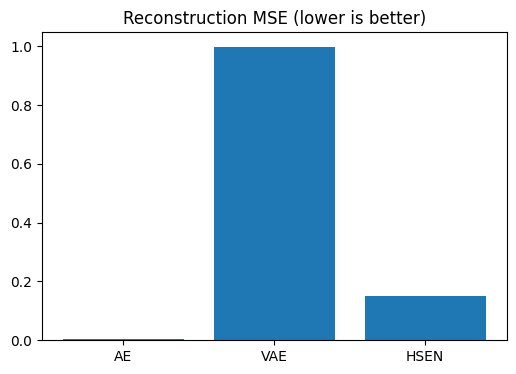
\includegraphics[width=0.72\linewidth]{fig_recon_mse.png}
  \caption{Reconstruction MSE comparison (lower is better).}
  \label{fig:mse}
\end{figure}

\begin{figure}[h!]
  \centering
  \begin{subfigure}{0.48\linewidth}
    \centering
    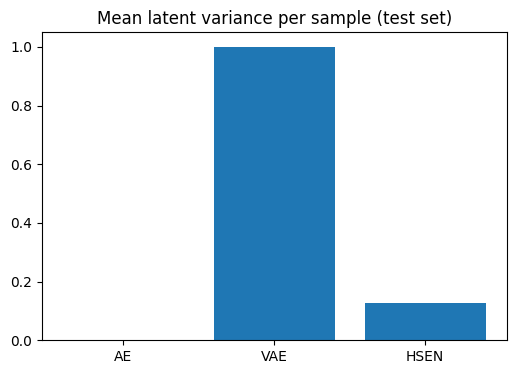
\includegraphics[width=\linewidth]{fig_latent_variance.png}
    \caption{Mean latent variance per sample.}
    \label{fig:latvar}
  \end{subfigure}\hfill
  \begin{subfigure}{0.48\linewidth}
    \centering
    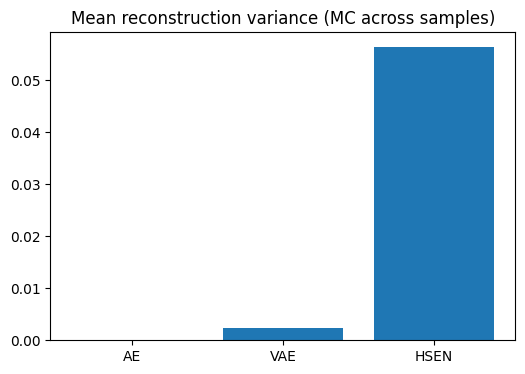
\includegraphics[width=\linewidth]{fig_recon_variance.png}
    \caption{MC reconstruction variance.}
    \label{fig:recvar}
  \end{subfigure}
  \caption{Uncertainty summaries for AE, VAE, HSEN.}
  \label{fig:uncertainty}
\end{figure}

\begin{figure}[h!]
  \centering
  \begin{subfigure}{0.32\linewidth}
    \centering
    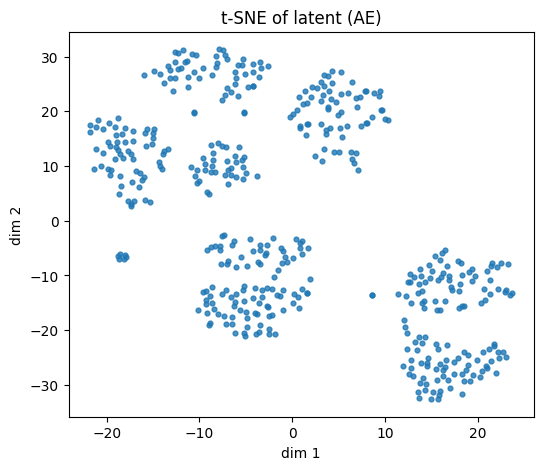
\includegraphics[width=\linewidth]{fig_tsne_ae.png}
    \caption{t-SNE (AE).}
  \end{subfigure}
  \begin{subfigure}{0.32\linewidth}
    \centering
    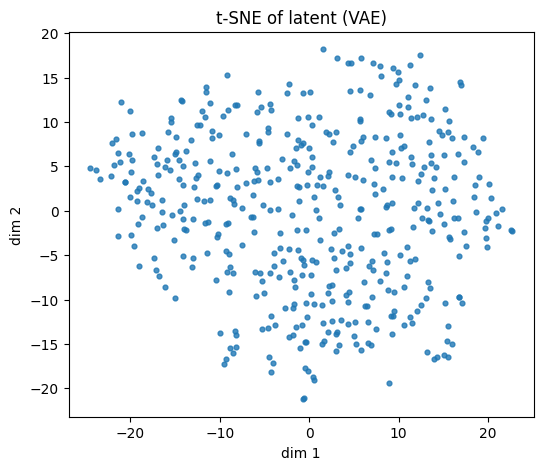
\includegraphics[width=\linewidth]{fig_tsne_vae.png}
    \caption{t-SNE (VAE).}
  \end{subfigure}
  \begin{subfigure}{0.32\linewidth}
    \centering
    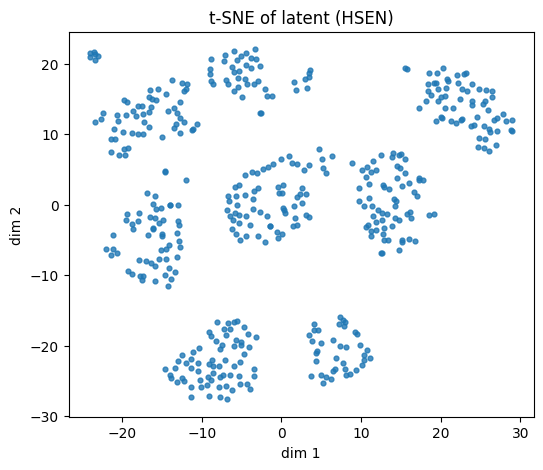
\includegraphics[width=\linewidth]{fig_tsne_hsen.png}
    \caption{t-SNE (HSEN).}
  \end{subfigure}
  \caption{Latent space visualization via t-SNE. HSEN and AE form compact groupings; VAE is diffuse.}
  \label{fig:tsne}
\end{figure}

% --- Force all figures above this point ---
\FloatBarrier 

\subsection{Qualitative \& Uncertainty Analysis}
t-SNE visualizations (Fig.~\ref{fig:tsne}) show that AE and HSEN produce compact, well-separated clusters, whereas VAE is diffuse. Latent variance is near zero for AE (deterministic), moderate for HSEN ($\sim 0.12$) indicating useful uncertainty, and high but uninformative for VAE. Although HSEN exhibits higher Monte Carlo reconstruction variance than AE, it achieves far lower MSE than VAE (Fig.~\ref{fig:mse}), indicating calibrated stochasticity around accurate reconstructions.

\subsection{Failure Cases}
\label{subsec:failure-cases}
\textbf{VAE posterior collapse:}
On this tabular dataset, the VAE sometimes collapses toward the prior, yielding diffuse latents and high reconstruction error; symptoms include small $\|\mu\|$ and large KL with weak mutual information.
\textbf{HSEN variance sensitivity:}
If $\lambda_{stab}$ is set too low, HSEN behaves like a VAE and loses clusterability; if too high, it overcontracts $z$ and harms reconstruction. A moderate value (\(0.1\)) balanced both.
\textbf{Cluster count mismatch:}
$k$-means can be unstable if $k$ is under/over-estimated; although we report stability NMI across seeds, mis-specified $k$ reduces silhouette.
\textbf{Outliers:}
Rare extreme points inflate reconstruction variance and may attract spurious micro-clusters in the latent space; robust scaling or trimming mitigates this.
\textbf{Deterministic baseline limits:}
AE achieves the best MSE but offers no uncertainty; for tasks requiring calibrated confidence, this is a practical failure mode despite strong reconstructions.


% ---------------- Discussion ----------------
\section{Discussion}
\textbf{AE} provides the best pure reconstruction on this tabular dataset but cannot express uncertainty. \textbf{VAE} underperforms due to over-regularization/posterior collapse. \textbf{HSEN} balances reconstruction, structure preservation (trustworthiness/continuity), and uncertainty, and yields more stable $k$-means clustering than VAE.

\paragraph{Theoretical implications:}
Let $z=\mu_\phi(x)+\epsilon\odot\sigma_\phi(x)$ with $\epsilon\!\sim\!\mathcal{N}(0,I)$. 
HSEN augments the VAE objective with a stability term $\|z_1-z_2\|^2$ for two conditionally i.i.d.\ samples $z_1,z_2\!\sim\!q_\phi(z\mid x)$.
Since $\mathbb{E}\|z_1-z_2\|^2 = 2\,\mathrm{tr}\,\mathrm{Var}[z\mid x]$, minimizing this term shrinks conditional variance without forcing $\mu_\phi(x)$ to the prior (in contrast to increasing $\beta$).
This yields \emph{tighter local neighborhoods} in latent space, improving trustworthiness/continuity and stabilizing $k$-means, while retaining a non-zero $\sigma_\phi(x)$ that encodes calibrated uncertainty.


\subsection{Limitations and Obstacles}
\begin{itemize}
  \item No ground-truth cluster labels $\Rightarrow$ ARI/NMI vs.\ labels not reported.
  \item HSEN adds modest compute (double sampling).
  \item Reconstruction variance for HSEN is higher than AE, which may affect tasks prioritizing deterministic reconstructions.
\end{itemize}

\subsection{Future Work}
\begin{itemize}
  \item Image datasets with generative metrics (FID/IS).
  \item Mixture/hierarchical priors or contrastive regularizers to improve separation.
  \item Semi-supervised CKD stage prediction as a downstream probe.
\end{itemize}

% ---------------- Conclusion ----------------
\section{Conclusion}
HSEN, a non-deterministic embedding model with a stability regularizer, outperforms VAE on reconstruction, trustworthiness, continuity, and clustering stability, while providing meaningful uncertainty estimates. AE remains strongest for raw MSE, but HSEN offers a better trade-off for exploratory and robust unsupervised analysis on tabular data.

% ---------------- References ----------------
\begin{thebibliography}{9}

\bibitem{kingma2013auto}
D.~P. Kingma and M.~Welling.
\newblock Auto-Encoding Variational Bayes.
\newblock \emph{arXiv preprint arXiv:1312.6114}, 2013.

\bibitem{higgins2016beta}
I.~Higgins et~al.
\newblock Beta-VAE: Learning Basic Visual Concepts with a Constrained Variational Framework.
\newblock \emph{ICLR Workshop}, 2017.

\bibitem{xie2016unsupervised}
J.~Xie, R.~Girshick, and A.~Farhadi.
\newblock Unsupervised Deep Embedding for Clustering Analysis.
\newblock \emph{ICML}, 2016.

\end{thebibliography}

\end{document}

